\documentclass{article}
	
\usepackage[margin=1in]{geometry}		% For setting margins
\usepackage{amsmath}				% For Math
\usepackage[]{amssymb}
\usepackage{amsmath}
\usepackage{gensymb}
\usepackage{fancyhdr}				% For fancy header/footer
\usepackage{graphicx}				% For including figure/image
\usepackage{cancel}					% To use the slash to cancel out stuff in work
\usepackage{wasysym}                % For cent symbol
\usepackage{pgfplots}
\usepackage{gnuplottex}

\pgfplotsset{width=7cm,compat=newest}
\usepgfplotslibrary{fillbetween}

% We will externalize the figures
% \usepgfplotslibrary{external}
% \tikzexternalize

%%%%%%%%%%%%%%%%%%%%%%
% Set up fancy header/footer
\pagestyle{fancy}
\fancyhead[RO,R]{{\textbf{Andry Paez}}}
\fancyhead[LO,L]{\textbf{Ch.14}}
\fancyhead[CO,C]{\textbf{Problem Set 1}}
% \fancyhead[RO,R]{\today}
\fancyfoot[LO,L]{}
\fancyfoot[CO,C]{\thepage}
\fancyfoot[RO,R]{}
\renewcommand{\headrulewidth}{0.4pt}
\renewcommand{\footrulewidth}{0.4pt}
%%%%%%%%%%%%%%%%%%%%%%

\newcommand{\hmwkTitle}{Ch 14 - Problem Set 1}
% \newcommand{\hmwkDueDate}{February 12, 2014}
\newcommand{\hmwkClass}{Calculus 3}
% \newcommand{\hmwkClassTime}{}
% \newcommand{\hmwkClassInstructor}{Professor Isaac Newton}
\newcommand{\hmwkAuthorName}{\textbf{Andry Paez}}

% math commands
\newcommand{\ihat}{\;\hat{\textbf{\i}}}
\newcommand{\jhat}{\;\hat{\textbf{\j}}}
\newcommand{\khat}{\;\hat{\textbf{k}}}
\newcommand{\rvec}{\vec{r}(t)}
\newcommand{\drvec}{\vec{r}\;'(t)}
\newcommand\vv[1]{\langle #1 \rangle}
\newcommand\vc[2]{\vec{#1}(#2)}
\newcommand\vcd[2]{\vec{#1}\;'(#2)}
\newcommand\vcdd[2]{\vec{#1}\;''(#2)}
\newcommand\vcddd[2]{\vec{#1}\;'''(#2)}
\newcommand\mgv[1]{\|#1\|}
\newcommand\mgvv[2]{\sqrt{\left(#1\right)^2 + \left(#2\right)^2}}
\newcommand\mgvvv[3]{\sqrt{\left(#1\right)^2 + \left(#2\right)^2 + \left(#3\right)^2}}
\newcommand\rr{\quad\Rightarrow\quad}
\newcommand{\limit}[4]{\lim_{(#1, #2) \to (#3, #4)}}
\newcommand{\limi}[2]{\lim_{#1 \to #2}}
\newcommand{\such}{\; | \;}
\newcommand{\lh}{\overset{L'H}{=}}
%
% Title Page
%
\title{
    \vspace{3in}
    \textmd{\textbf{\hmwkTitle}}\\
    \vspace{0.5in}
    \textmd{\textbf{\hmwkClass}}\\
    % \normalsize\vspace{0.1in}\small{Due\ on\ \hmwkDueDate\ at 3:10pm}\\
    % \vspace{0.1in}\large{\textit{\hmwkClassInstructor\ \hmwkClassTime}}
    \vspace{4in}
}

\author{\hmwkAuthorName}
\date{}

\begin{document}
\maketitle

% New blank page for printers that print on both sides of paper
\clearpage\shipout\null

\begin{center}
    \section*{\underline{Section 1: Functions of Several Variables}}
\end{center}

\subsection*{3. Let $g(x,y) = x^2\ln (x+y)$ \\ (\textit a) Evaluate $g(3, 1)$. \\ (\textit b) Find and sketch the domain of $g$. \\ (\textit c) Find the range of $g$.}
\centerline{\textbf{Solution}}
\begin{align*}
    \intertext{\textit a) 9\ln 4}
    \intertext{\textit b) $D:\{(x,y) \such y > -x\}$}
    % graph and shade region of domain
    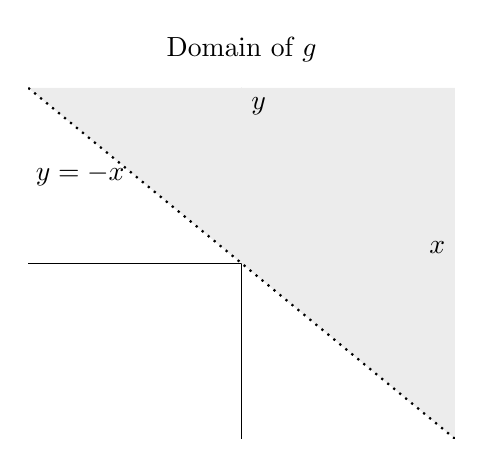
\begin{tikzpicture}
        \begin{axis} [
            title={Domain of $g$},
            axis lines=middle,
            xlabel=$x$,
            ylabel=$y$,
            ymin=-5, ymax=5,
            ticks=none,
        ]
        \addplot [
            name path=line,
            domain=-5:5,
            dotted,
            thick,
        ]
        {-x} node [left, pos=0.25] {$y=-x$};];  
        \addplot[draw=none, name path=axis] {5};
        \addplot [fill=gray!15] fill between[of=line and axis];
        \end{axis}
    \end{tikzpicture}
    \intertext{\textit c) $\mathbb R$}
\end{align*}
\subsection*{7 - 15 (odd)}

Find and sketch the domain of the function.

\subsubsection*{7. $f(x,y)=\sqrt{x-2} + \sqrt{y-1}$}
\centerline{\textbf{Solution}}
\begin{align*}
    \intertext{$D:\{(x,y)\such x\geq 2, y\geq 1\}$}
    \begin{tikzpicture}
        % Define the axis
        \draw[->] (-1,0) -- (5,0) node[right] {$x$};
        \draw[->] (0,-1) -- (0,5) node[above] {$y$};
        % Draw the lines 
        \draw (2, 5) -- (2, -1)
        \draw (-1, 1) -- (5, 1) 
        % Shade the region x >= 2 and y >= 1
        \fill[gray!15] (2,1) rectangle (5,5);
    \end{tikzpicture}
\end{align*}
\subsubsection*{9. $q(x,y)=\sqrt x + \sqrt{4- 4x^2 - y^2}$}
\centerline{\textbf{Solution}}
\begin{align*}
    \intertext{$D:\{(x,y)\such x^2+\frac 1 4 y^2\leq 1, x\geq 0\}$}
    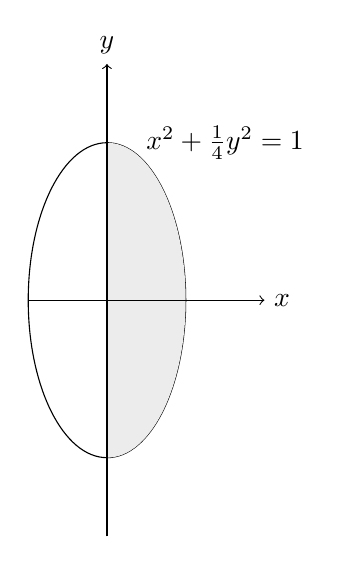
\begin{tikzpicture}
        % Draw the  ellipse 
        \draw (0, 0) ellipse (1 and 2); 
        \node at (1.5, 2) {$x^2 + \frac 1 4 y^2 = 1$};
        % Define a custom clip path to fit the inside of the ellipse
        \begin{scope}
            \clip (0,-2) -- (2,-2) -- (2,0) -- (2,2) -- (0,2) -- cycle;
            % Shade the region
            \fill[gray!15] (0,0) ellipse (1 and 2);
        \end{scope}
        % Define the axis
        \draw[->] (-1,0) -- (2,0) node[right] {$x$};
        \draw[->] (0,-3) -- (0,3) node[above] {$y$};
    \end{tikzpicture}
\end{align*}
\subsubsection*{11. $g(x,y) = \displaystyle\frac{x - y}{x + y}$}
\centerline{\textbf{Solution}}
\begin{align*}
    \intertext{$D:\{(x,y)\such y\neq -x\}$}
    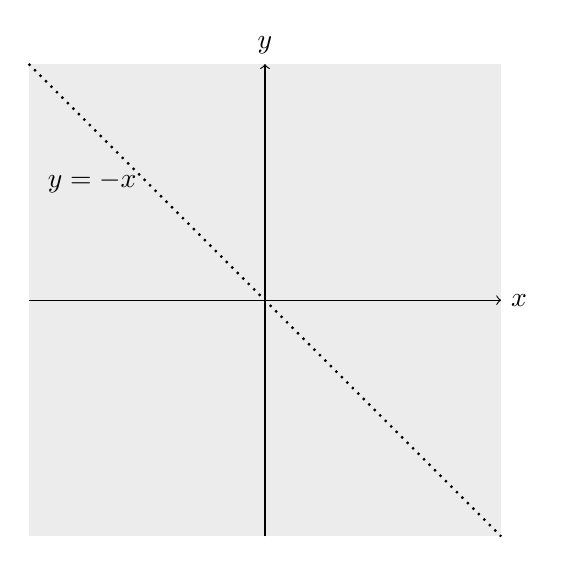
\begin{tikzpicture}
        % Shade the region y != -x
        \fill[gray!15] (-3,-3) -- (-3,3) -- (3,3) -- (3,-3) -- cycle;
        % Draw the lines 
        \draw[dotted, thick] (-3, 3) -- (3,-3) node [left, pos=0.25] {$y=-x$};
        % Define the axis
        \draw[->] (-3,0) -- (3,0) node[right] {$x$};
        \draw[->] (0,-3) -- (0,3) node[above] {$y$};
    \end{tikzpicture}
\end{align*}
\subsubsection*{13. $p(x,y) = \displaystyle\frac{\sqrt{xy}}{x+1}$}
\centerline{\textbf{Solution}}
\begin{align*}
    \intertext{$D:\{(x,y)\such x\neq 0, xy\geq 0\}$}
    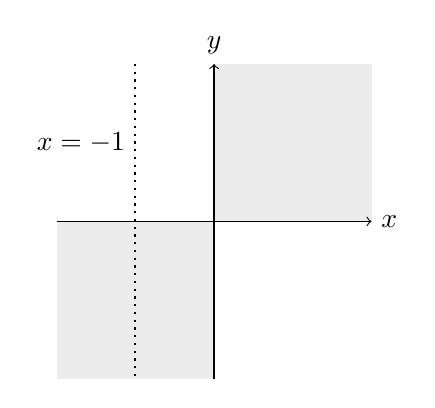
\begin{tikzpicture}
        % Shade the region xy >= 0
        \fill [gray!15] (0,0) -- (0,2) -- (2,2) -- (2,0) -- cycle;
        \fill [gray!15] (0,0) -- (0,-2) -- (-2,-2) -- (-2,0) -- cycle;
        % Draw the line x != -1
        \draw[dotted, thick] (-1,2) -- (-1,-2) node [left, pos=0.25] {$x=-1$};
        % Define the axis
        \draw[->] (-2,0) -- (2,0) node[right] {$x$};
        \draw[->] (0,-2) -- (0,2) node[above] {$y$};
    \end{tikzpicture}
\end{align*}
\subsubsection*{15. $f(x,y,z) = \sqrt{4 - x^2} + \sqrt{9 - y^2} + \sqrt{1 - z^2}$}
\centerline{\textbf{Solution}}
\begin{align*}
    \intertext{$D:\{(x, y, z)\such -2 \leq x \leq 2, -3 \leq y \leq 3, -1 \leq z \leq 1\}$}   
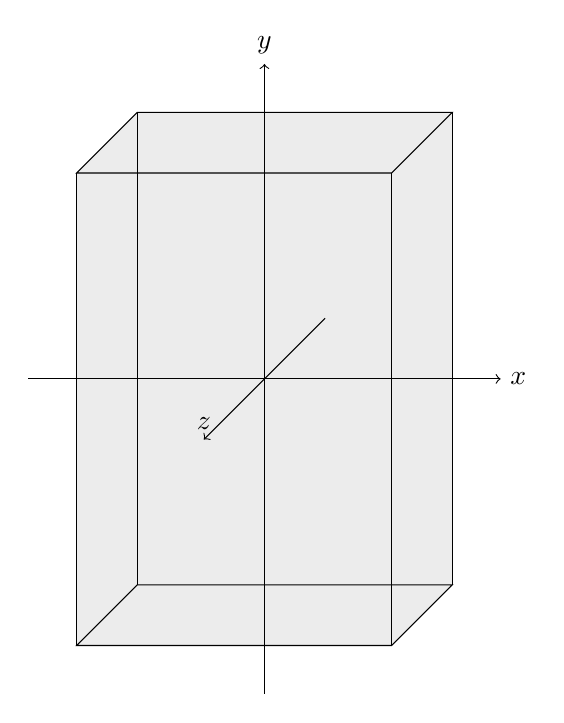
\begin{tikzpicture}
    % Define the coordinates of the vertices of the rectangular prism
    \coordinate (A) at (2,3,1);
    \coordinate (B) at (2,3,-1);
    \coordinate (C) at (-2,3,-1);
    \coordinate (D) at (-2,3,1);
    \coordinate (E) at (2,-3,1);
    \coordinate (F) at (2,-3,-1);
    \coordinate (G) at (-2,-3,-1);
    \coordinate (H) at (-2,-3,1);
    % Shade the cube faces
    % Square faces 
    \fill[gray!15] (A) -- (B) -- (C) -- (D) -- cycle;
    \fill[gray!15] (E) -- (F) -- (G) -- (H) -- cycle;
    % Rectangle faces
    \fill[gray!15] (A) -- (E) -- (F) -- (B) -- cycle;
    \fill[gray!15] (D) -- (H) -- (G) -- (C) -- cycle;
    \fill[gray!15] (D) -- (A) -- (E) -- (H) -- cycle;
    \fill[gray!15] (C) -- (B) -- (F) -- (G) -- cycle;
    % Draw the edges of the cube
    \draw (A) -- (B) -- (C) -- (D) -- cycle;
    \draw (E) -- (F) -- (G) -- (H) -- cycle;
    \draw (A) -- (E);
    \draw (B) -- (F);
    \draw (C) -- (G);
    \draw (D) -- (H);
    % Define the axis
    \draw[->] (-3,0,0) -- (3,0,0) node[right] {$x$};
    \draw[->] (0,-4,0) -- (0,4,0) node[above] {$y$};
    \draw[->] (0,0,-2) -- (0,0,2) node[above] {$z$};
\end{tikzpicture}
\end{align*}
\subsection*{17. A model for the surface area of a human body is given by the function \\
    \begin{align*} S = f(w, h) = 0.1091w^{0.425}h^{0.725} \end{align*} \\
    where $w$ is the weight (in pounds), $h$ is the height (in inches), and $S$ is measured in square feet. \\
    (\textit a) Find $f(160, 70)$ and interpret it. \\
    (\textit b) What is your own surface area?
$}
\centerline{\textbf{Solution}}
\begin{align*}
    \intertext{\textit a)}
    f(160, 70) = 0.1091(160^{0.425})(70^{0.725}) \approx 20.5 \\ 
    \intertext{The surface area of a human body that weighs 160 pounds and is 70 inches tall is about 20.5 square feet.}
\end{align*}
\subsection*{23 - 31 (odd)}
Sketch the graph of the function
\subsubsection*{23. $f(x,y) = y$}
\centerline{\textbf{Solution}}
\begin{align*}
    \intertext{This is an equation of the plane that goes through the origin and is parallel to the $x$-axis.}
    % \begin{tikzpicture}
    %     \begin{axis}[
    %         title={$f(x,y) = y$},
    %         axis lines=box,
    %         xlabel=$x$,
    %         ylabel=$y$,
    %         zlabel=$z$,
    %     ]
    %     \addplot3 [
    %         domain=-2:2,
    %         samples=50,
    %         mesh,
    %         colormap/blackwhite,
    %     ]
    %     {y};
    %     \end{axis} 
    % \end{tikzpicture}
\end{align*}
\subsubsection*{25. $f(x,y) = 10 - 4x -5y$}
\centerline{\textbf{Solution}}
\begin{align*}
    \intertext{Let $x=y=0 \rr z = 10$,\quad $x = z = 0 \rr y = 2$,\quad $y = z = 0 \rr x = 2.5$}
    \intertext{This is an equation of a plane that goes through the points $(0,0,10), (0,2,0), (2.5,0,0)$ [imagine it is shaded in].}
    % \begin{tikzpicture}
    %     \begin{axis}[
    %         title={$f(x,y) = 10 - 4x -5y$},
    %         axis lines=middle,
    %         xlabel=$x$,
    %         ylabel=$y$,
    %         zlabel=$z$,
    %         view={135}{45},
    %     ]
    %     \addplot3[
    %         name path=plane,
    %         mesh,
    %         colormap/blackwhite,
    %     ] 
    %     coordinates {
    %         (0,0,0) (0,0,10) (0,2,0) (2.5,0,0) (0,0,10)
    %     };
    %     \addplot3[
    %         name path =origin,
    %         draw=none
    %     ]
    %     {0};
    % \end{axis}
    % \end{tikzpicture}
\end{align*}
\subsubsection*{27. $f(x,y) = \sin x$}
\centerline{\textbf{Solution}}
\begin{align*}
    % \intertext{This is an equation of a cylinder that goes through the origin and is parallel to the $x$-axis}
    % \begin{tikzpicture}
    %     \begin{axis}[
    %         title={$f(x,y) = \sin x$},
    %         axis lines=middle,
    %         xlabel=$x$,
    %         ylabel=$y$,
    %         zlabel=$z$,
    %     ]
    %     \addplot3 [
    %         mesh,
    %         samples=50,
    %         colormap/blackwhite
    %     ]
    %     {sin(deg(x))};
    %     \end{axis} 
    % \end{tikzpicture}
\end{align*}
\subsubsection*{29. $f(x,y) = x^2 + 4y^2 + 1$}
\centerline{\textbf{Solution}}
\begin{align*}
    \intertext{This is an equation of an elliptic paraboloid that goes through the origin and is parallel to the $z$-axis.}
    \begin{tikzpicture}
        \begin{axis}[
            axis lines=middle,
            xlabel={$y$},
            ylabel={$z$},
            xlabel style={below right},
            ylabel style={above left},
            xmin=-5.5,
            xmax=5.5,
            ymin=-5.5,
            ymax=5.5,
            ticks=none,
            scale=1.5,
        ]
        \addplot [mark=none,domain=-4:4] {x} node [pos=0.0, left] {$x$};
        \end{axis}
    \end{tikzpicture}
\end{align*}
\subsubsection*{31. $f(x,y) = \sqrt{4 - 4x^2 - y^2}$}
\centerline{\textbf{Solution}}
\begin{align*}
    \intertext{This is the top half of ellipsoid}
    % \begin{tikzpicture}
    %     \begin{axis} [
    %         title={$f(x,y) = \sqrt{4 - 4x^2 - y^2}$},
    %         axis lines=middle,
    %         xlabel=$x$,
    %         ylabel=$y$,
    %         zlabel=$z$,
    %     ] 
    %     \addplot3 [
    %         surf,
    %         samples=50,
    %         colormap/blackwhite,
    %     ] 
    %     {sqrt(4 - 4*x^2 - y^2)};
    %     \end{axis}
    % \end{tikzpicture}
\end{align*}
% Needs graphs or screenshot and insert as figure
\subsection*{32. Match the function with its graph (labeled I–VI). Give reasons for your choices. \\
    (\textit a) $f(x,y) = \displaystyle\frac 1 {1 + x^2 + y^2} \qquad (\textit b)\; f(x,y) = \frac 1 {1 + x^2 y^2}$ \\\\
    (\textit c) $f(x,y) = \ln (x^2 + y^2) \qquad \;(\textit d)\; f(x,y) = \cos \sqrt{x^2 + y^2}$ \\\\
    (\textit e) $f(x,y) = |xy| \qquad \qquad \quad (\textit f)\; f(x,y) = \cos (xy)$\\
}
% \begin{tikzpicture}
%     \begin{axis}[
%         title={I},
%         axis lines=middle,
%         xlabel=$x$,
%         ylabel=$y$,
%         zlabel=$z$,
%         xmin=-4, xmax=4,
%         ymin=-4, ymax=4,
%         zmin=0, zmax=1.5,
%         view={135}{45},
%         ticks = none,
%         colormap/hot2,
%         ]
%         \addplot3[
%             surf,
%             samples = 50,
%             domain=-3:3,
%         ] {1/(1+ x^2 * y^2)};
%     \end{axis} 
% \end{tikzpicture}
% \begin{tikzpicture}
%     \begin{axis}[
%         title={II},
%         axis lines=middle,
%         xlabel=$x$,
%         ylabel=$y$,
%         zlabel=$z$,
%         % xmin= -5, xmax= 5,
%         % ymin= -5, ymax= 5,
%         % zmin= 0, zmax= 5,
%         view={110}{45},
%         ticks = none,
%         colormap/hot2,
%         ]
%         \addplot3[
%             surf,
%             samples = 50,
%             domain= -3 : 3,
%             domain y = -3 : 3,
%         ] {cos(deg(x*y))};
%     \end{axis} 
% \end{tikzpicture}
% \begin{tikzpicture}
%     \begin{axis}[
%         title={III},
%         axis lines=middle,
%         xlabel=$x$,
%         ylabel=$y$,
%         zlabel=$z$,
%         xmin=-4, xmax=4,
%         ymin=-4, ymax=4,
%         zmin=0, zmax=1.5,
%         view={135}{30},
%         ticks = none,
%         colormap/hot2,
%         ]
%         \addplot3[
%             surf,
%             samples = 50,
%             domain=-3:3,
%         ] {1/(1+x^2+y^2)};
%     \end{axis} 
% \end{tikzpicture}
% \begin{tikzpicture}
%     \begin{axis}[
%         title={IV},
%         axis lines=middle,
%         xlabel=$x$,
%         ylabel=$y$,
%         zlabel=$z$,
%         xmin=-5, xmax=5,
%         ymin=-5, ymax=5,
%         zmin=-0.5, zmax=3,
%         view={135}{45},
%         ticks = none,
%         colormap/hot2,
%         ]
%         \addplot3[
%             surf,
%             samples = 50,
%             domain=-5:5,
%         ] {ln(x^2 + y^2)};
%     \end{axis} 
% \end{tikzpicture}
% \begin{tikzpicture}
%     \begin{axis}[
%         title={V},
%         axis lines=middle,
%         xlabel=$x$,
%         ylabel=$y$,
%         zlabel=$z$,
%         % xmin=-5, xmax=5,
%         % ymin=-5, ymax=5,
%         % zmin=0, zmax=4,
%         view={110}{45},
%         ticks = none,
%         colormap/hot2
%         ]
%         \addplot3[
%             surf,
%             samples = 50,
%             domain=-4:4,
%         ] {cos(deg(sqrt(x^2 + y^2)))};
%     \end{axis} 
% \end{tikzpicture}
% \begin{tikzpicture}
%     \begin{axis}[
%         title={VI},
%         axis lines=middle,
%         xlabel=$x$,
%         ylabel=$y$,
%         zlabel=$z$,
%         xmin= -5, xmax= 5,
%         ymin= -5, ymax= 5,
%         zmin= 0, zmax= 20,
%         view={110}{45},
%         ticks = none,
%         colormap/hot2,
%         ]
%         \addplot3[
%             surf,
%             samples = 50,
%             domain= -5 : 5,
%             domain z = 0 : 20,
%         ] {abs(x*y)};
%     \end{axis} 
% \end{tikzpicture}
\\
\centerline{\textbf{Solution}}

\begin{align*}
    \intertext{\textit a)}
    \intertext{The graph of $f(x,y) = \displaystyle\frac 1 {1 + x^2 + y^2}$ is III}
    \intertext{When $x = y = 0 \rr z = 1$, so the graph intersects the $z$-axis at $(0,0,1)$.}
    \intertext{If we solve for the $zx$ and $zy$ planes we get $z = \displaystyle\frac 1 {1 + x^2}$ and $z = \displaystyle\frac 1 {1 + y^2}$ respectively.}
    \intertext{\textit{b)}}
    \intertext{The graph of $f(x,y) = \displaystyle\frac 1 {1 + x^2 y^2}$ is I}
    \intertext{When $x = y = 0 \rr z = 1$, so the graph intersects the $z$-axis at $(0,0,1)$.}
    \intertext{Let $x = 1$ and then we solve for $z = \lim_{y \to \infty} \displaystyle\frac 1 {1 + y^2} = 0$. For graph I, if we gauge the $x = 1$ position and move up the $y$ axis, we can see that $z$ does indeed approach a value like 0.}
    \intertext{\textit{c)}}
    \intertext{The graph of $f(x,y) = \ln (x^2 + y^2)$ is IV}
    \intertext{When $x = y = 0$ z is undefined}
    \intertext{The only graph that seems to have a hole at the origin is IV.}
    \intertext{\textit{d)}} 
    \intertext{The graph of $f(x,y) = \cos \sqrt{x^2 + y^2}$ is V}
    \intertext{When $x = y = 0 \rr z = 1$, so the graph intersects the $z$-axis at $(0,0,1)$.}
    \intertext{When $x = 0$ and $y=0$ then $z=\cos y$ and $z=\cos x$ respectively.}
    \intertext{The only graph that has a point at $(0,0,1)$ and has sinusoidal movement when $(0, (\text{y or x}) \to \infty, -1 \leq z \leq 1)$ is V.}
    \intertext{\textit{e)}}
    \intertext{The graph of $f(x,y) = |xy|$ is VI}
    \intertext{When $x = y = 0 \rr z = 0$, so the graph intersects the $z$-axis at $(0,0,0)$.}
    \intertext{Out of the remaining graphs, the only graph that seems like it has an intersection at the origin is VI.}
    \intertext{\textit{f)}}
    \intertext{The graph of $f(x,y) = \cos (xy)$ is II}
    \intertext{Process of elimination :) (please don't dock me points for this)}
\end{align*}
\newpage
\subsection*{33. A contour map for a function $f$ is shown. Use it to estimate the values of $f(-3, 3)$ and $f(3, -2)$. What can you say about the shape of the graph?}

\begin{figure}[h]
    \begin{center}
        \includegraphics[width=0.5\textwidth]{figures/33.png}
    \end{center}
\end{figure}

\centerline{\textbf{Solution}}
\begin{align*}
    \intertext{Looking at the contour map, it seems that $f(-3, 3)$ is $\approx$ 56 because it is between the 50 and 60 but a little closer to the 60.} 
    \intertext{$f(3, -2)$ seems like it is $\approx$ 35 because it is in the middle of 40 and 35} 
    \intertext{The shape of the graph seems like a hill or the top half of an ellipsoid} 
\end{align*}
\newpage
\subsection*{45, 47 \& 51}

Draw a contour map of the function showing several level curves.

\subsubsection*{45. $f(x,y) = x^2 - y^2$}
\centerline{\textbf{Solution}}
\begin{align*}
    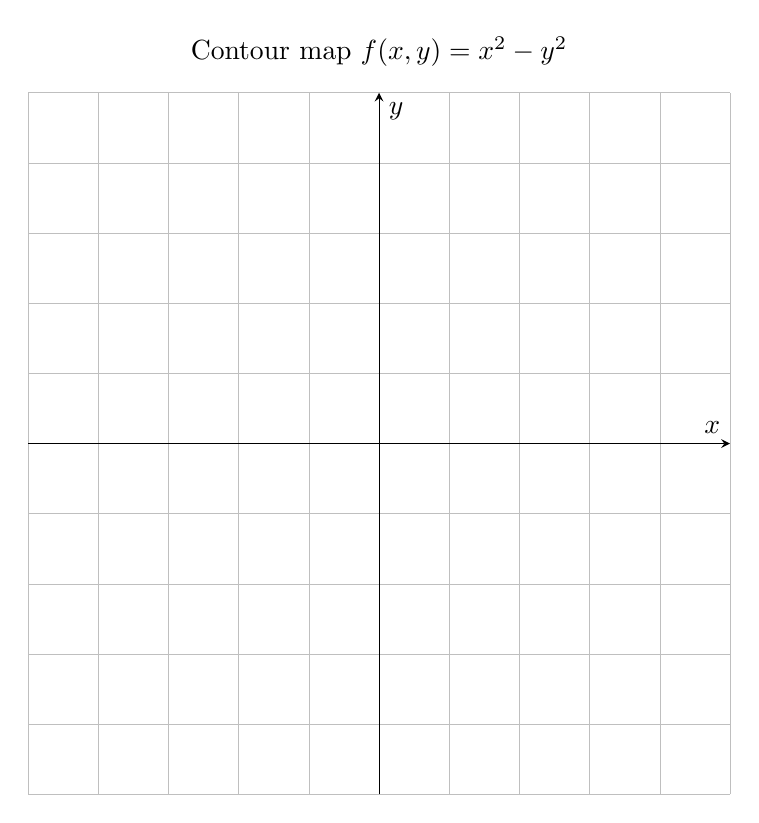
\begin{tikzpicture}
        \begin{axis} [
            title={Contour map $f(x,y) = x^2 - y^2$},
            axis lines=middle,
            axis equal image,
            xlabel=$x$,
            ylabel=$y$,
            xmin=-10, xmax=10,
            ymin=-10, ymax=10,
            grid=both,
            grid style = {line width = .1pt, draw = gray!10},
            major grid style = {line width = .2pt, draw = gray!50},
            ticks=none,
            scale=2.0,
        ]
       \end{axis} 
    \end{tikzpicture}
\end{align*}

\subsubsection*{47. $f(x,y) = \sqrt x + y$}
\centerline{\textbf{Solution}}
\begin{align*}
    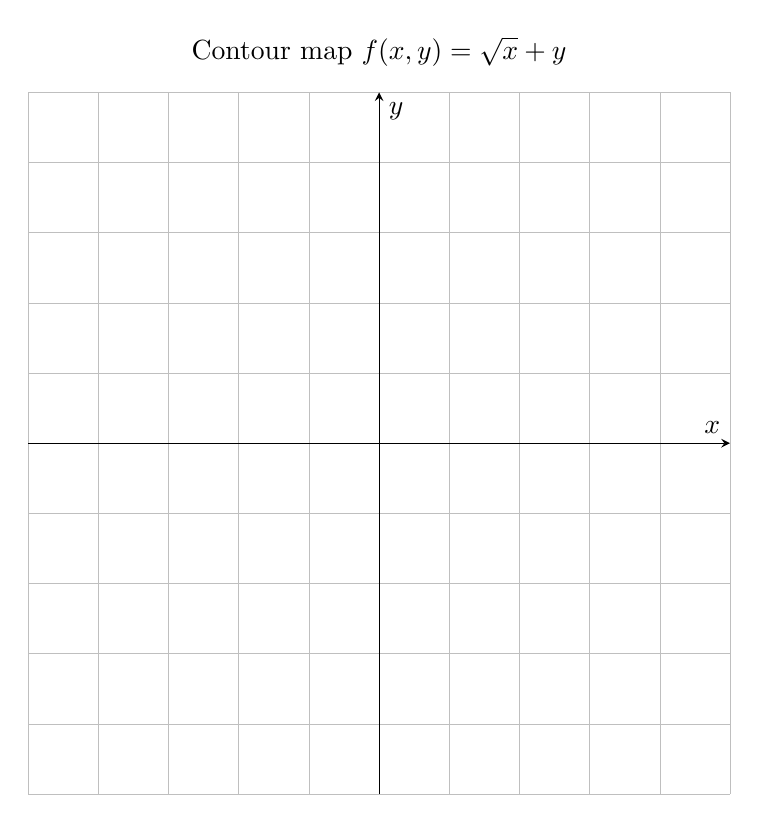
\begin{tikzpicture}
        \begin{axis} [
            title={Contour map $f(x,y) = \sqrt x + y$},
            axis lines=middle,
            axis equal image,
            xlabel=$x$,
            ylabel=$y$,
            xmin=-10, xmax=10,
            ymin=-10, ymax=10,
            grid=both,
            grid style = {line width = .1pt, draw = gray!10},
            major grid style = {line width = .2pt, draw = gray!50},
            ticks=none,
            scale=2.0,
        ]
       \end{axis} 
    \end{tikzpicture}
\end{align*}
% broken, won't compile
\subsubsection*{51. $f(x,y) = \sqrt{x^2 + y^2}$}
\centerline{\textbf{Solution}}
\newpage
\begin{align*}
    \begin{tikzpicture}
        \begin{axis} [
            title={Contour map $f(x,y) = \sqrt{x^2 + y^2}$,
            axis lines=middle,
            axis equal image,
            xlabel=$x$,
            ylabel=$y$,
            xmin=-10, xmax=10,
            ymin=-10, ymax=10,
            grid=both,
            grid style = {line width = .1pt, draw = gray!10},
            major grid style = {line width = .2pt, draw = gray!50},
            ticks=none,
            scale=2.0,
        ]
       \end{axis} 
    \end{tikzpicture}
\end{align*}

\subsection*{53. Sketch both a contour map and a graph of the given function and compare them.}

$$f(x,y) = x^2 + 9y^2$$

\centerline{\textbf{Solution}}
\begin{align*}
    \begin{tikzpicture}
        \begin{axis} [
            title={Contour map $f(x,y) = x^2 + 9y^2}$,
            axis lines=middle,
            axis equal image,
            xlabel=$x$,
            ylabel=$y$,
            xmin=-10, xmax=10,
            ymin=-10, ymax=10,
            grid=both,
            grid style = {line width = .1pt, draw = gray!10},
            major grid style = {line width = .2pt, draw = gray!50},
            ticks=none,
            scale=2.0,
        ]
       \end{axis} 
    \end{tikzpicture}
\end{align*}
\begin{align*}
    \begin{tikzpicture}
        \begin{axis}[
            axis lines=middle,
            xlabel={$y$},
            ylabel={$z$},
            xlabel style={below right},
            ylabel style={above left},
            xmin=-5.5,
            xmax=5.5,
            ymin=-5.5,
            ymax=5.5,
            ticks=none,
            scale=1.5,
        ]
        \addplot [mark=none,domain=-4:4] {x} node [pos=0.0, left] {$x$};
        \end{axis}
    \end{tikzpicture}
\end{align*}

\subsection*{61 - 66} 
Match the function (\textit a) with its graph (labeled A–F below) and (\textit b) with its contour map (labeled I–VI). Give reasons for your choices.

\begin{figure}[h] %h = here, t = top, b = bottom, p = page of figures
    \begin{center}
        \includegraphics[width=0.95\textwidth]{figures/61-66.jpg}
    \end{center}
\end{figure}

\subsubsection*{61. $z = \sin (xy)$}
\centerline{\textbf{Solution}}
\begin{align*}
    \intertext{It seems like the graph of $z = \sin (xy)$ is C}
    \intertext{When $x \to \infty$ and $y \to \infty$ then $-1 \leq z \leq 1$.}
    \intertext{In other words, at $45\degree, 135\degree, 235\degree, 315\degree$ in terms of $xy$, $z$ should be infinitely sinusoidal the farther you go out}
    \intertext{Since the function of $z$ is $\sin$ then the graph must intersect the $z$ at origin}
    \intertext{For the contour map, the graph that looks that follows this description is II}
\end{align*}
\subsubsection*{62. $z = e^x \cos y$}
\centerline{\textbf{Solution}}
\begin{align*}
    \intertext{When $x=y=0$ then $z=1 \rr (0,0,1)$.}
    \intertext{Setting $x = 0 \rr z = \cos y \rr (0, y \to \infty, -1 \leq z \leq 1)$ this just means that x is constant and as y increases/decreases towards either positive or negative infinity, z will be sinusoidal} 
    \intertext{Setting $y = 0 \rr z = e^x \rr (0, y \to \infty^+, \infty^+)(0, y \to \infty^-, 0)$ this just means that y is constant and depending if x is increasing or decreasing, z will increase exponentially to infinity or approach 0} 
    \intertext{$\therefore$ The graph that seems to follow this description is A and the associated contour map seems to be IV}
\end{align*}
\subsubsection*{63. $z = \sin (x-y)$}
\centerline{\textbf{Solution}}
\begin{align*}
    \intertext{The graph would have an intersection at the origin $x=y=0 \rr z=0$}
    \intertext{When $x = 0 \rr z = \sin (-y)$, so the function will first dip down to $z=-1$ in the zy-trace}
    \intertext{When $y = 0 \rr z = \sin (x)$, so the function will first go up to $z=1$ in the zx-trace}
    \intertext{$\therefore$ The graph that matches this description looks like F and the associated contour map seems to be I}
\end{align*}
\subsubsection*{64. $z = \sin x - \sin y$}
\centerline{\textbf{Solution}}
\begin{align*}
    \intertext{The graph would have an intersection at the origin $x=y=0 \rr z=0$}
    \intertext{$z = 1 - 1 = 0$ \quad\leftrightarrow\quad $x = y = n \cdot \frac \pi 2$, $\{n \in \mathbb{Z} \such n = 2k-1, k \in \mathbb{Z}\}$}
    \intertext{$z = 0 - 0 = 0$ \quad\leftrightarrow\quad $x = y = n \cdot \frac \pi 2$, $\{n \in \mathbb{Z} \such n = 2k, k \in \mathbb{Z}\}$}
    \intertext{This behavior appears symmetric with $z =0$ appearing at areas where $x = y$.}
    \intertext{$\therefore$ The graph that best matches this behavior is E and the associated contour map would be III}
\end{align*}
\subsubsection*{65. $z = (1-x^2)(1-y^2)$}
\centerline{\textbf{Solution}}
\begin{align*}
    \intertext{The graph would have an intersection at  $(0,0,1) \quad x=y=0 \rr z=1$}
    \intertext{If we look at the $zy$ and $zx$ traces, we see that it is a parabola opening down to negative $z$}
    \intertext{However, if we take $\limit x y \infty \infty (1-x^2)(1-y^2), \quad \{(x,y) \such x = y\}$ then we get $\infty$ where the graph, in this direction, would exponentially grow.}
    \intertext{$\therefore$ The graph that best fits this description would be B and the associated contour map would be VI.}
\end{align*}
\subsubsection*{66. $z = \displaystyle\frac{x-y}{1+ x^2+ y^2}$}
\centerline{\textbf{Solution}}
\begin{align*}
    \intertext{The graph would have an intersection at  $(0,0,0) \quad x=y=0 \rr z=0$}
    \intertext{Using process of elimination, the only graph left would be D and the associated contour map would be V.}
    \intertext{We could note its behavior in the $zy$ trace and see that $lim_{y \to \infty^+} \frac{-y}{1 + y^2} = 0$ with $z$ decreasing at first, vice versa with $zx$ trace}
    \intertext{To find the point at which $z$ is at a minimum when $y \to \infty^+$,}
    z &= -y(1+y^2)^{-1} \\
    \frac{dz}{dy} &= -\frac{1}{1+y^2} + \frac{2y^2}{(1+y^2)^{2}} \\
    0 &= -\frac{1}{1+y^2} + \frac{2y^2}{(1+y^2)^{2}} \\
    \frac{1}{1+y^2} &= \frac{2y^2}{(1+y^2)^{2}} \\
    1 &= \frac{2y^2}{1+y^2} \\
    1 + y^2 &= 2y^2 \\
    1 &= y^2 \\
    y &= \pm 1 = +1 \\
    \intertext{And it seems there would be a maximum at $y = -1$}
\end{align*}
\subsection*{67. Describe the level surfaces of the function. \\ \begin{align*} f(x, y, z) = 2y - z + 1 \end{align*}}
\centerline{\textbf{Solution}}
\begin{align*}
    \intertext{If we rearrange the function, $x-2y+z=1$ and we see that this is an equation of a plane. If we substitute $k$ for 1 and play around with its value (choosing 3-5 vals for k) then we see that no matter which value we pick, the planes will be parallel}
\end{align*}
\newpage
\begin{center}
    \section*{\underline{Section 2: Limits and Continuity}}
\end{center}
\subsection*{5 - 11 (odd)}
Find the limit
\subsubsection*{5. $\lim_{(x,y) \to (3,2)} (x^2 y^3 - 4y^2)$}
\centerline{\textbf{Solution}}
\begin{align*}
    \intertext{Using direct substitution,}
    (9)(8) - 4(4) &= 72-16=56
\end{align*}
\subsubsection*{7. $\limit x y {-3} 1 \displaystyle\frac{x^2 y - xy^3}{x - y + 2}$} 
\centerline{\textbf{Solution}}
\begin{align*}
    \intertext{Using direct substitution,}
    \frac{9(1) + 3(1^3)}{-3 - 1 + 2} &= \frac{12}{-2} = -6
\end{align*}
\subsubsection*{9. $\limit x y \pi {\pi/2} y \sin (x - y)$}
\centerline{\textbf{Solution}}
\begin{align*}
    \intertext{Using direct substitution,}
    \frac \pi 2 \sin (\pi - \frac \pi 2) &= \frac \pi 2 \sin (\frac \pi 2) = \frac \pi 2 (1) = \frac \pi 2 
\end{align*}
\subsubsection*{11. $\limit x y 1 1 \left(\displaystyle\frac{x^2 y^3 - x^3 y^2}{x^2 - y^2}\right) }
\centerline{\textbf{Solution}}
\begin{align*}
    \intertext{Let $x = 1$,}
    \limi x 1 \left(\displaystyle\frac{1^2 y^3 - 1^3 y^2}{1^2 - y^2}\right) &= \limi x 1 \left(\displaystyle\frac{y^3 - y^2}{1 - y^2}\right) \lh \limi x 1 \frac{3y^2 - 2y}{-2y} = \frac{1}{-2}\\
    \intertext{Let $y = 1$,}
    \limi y 1 \left(\displaystyle\frac{x^2 1^3 - x^3 1^2}{1^2 - y^2}\right) &= \limi y 1 \left(\displaystyle\frac{x^2 - x^3}{x^2 - 1}\right) \lh \limi x 1 \frac{2x - 3x^2}{2x} = \frac{-1}{2}\\
    \intertext{$\therefore$ The limit = $\frac 1 2}
\end{align*}

\subsection*{13 - 17 (odd)}
Show that the limit does not exist
\subsubsection*{13. $\limit x y 0 0 \displaystyle\frac {y^2}{x^2 + y^2}$}
\centerline{\textbf{Solution}}
\begin{align*}
    \intertext{Let $x = 0$,}
    \limi y 0 \displaystyle\frac{y^2}{y^2} &= 1 \\
    \intertext{Let $y = 0$,}
    \limi x 0 \displaystyle\frac{0}{x^2} &= 0\\
    \intertext{1 \neq 0 \quad  $\therefore$ The limit DNE}
\end{align*}
\subsubsection*{15. $\limit x y 0 0 \displaystyle\frac {(x+y)^2}{x^2 + y^2}$}
\centerline{\textbf{Solution}}
    \intertext{Let $y = x$,}
    \limi x 0 \displaystyle\frac {(x+x)^2}{x^2 + x^2} &= \limi x 0 \displaystyle\frac {4x^2}{2x^2} = 2 
    \intertext{Let $y = -x$,}
    \limi x 0 \displaystyle\frac {(0)^2}{x^2 + (-x)^2} &= \limi x 0 \displaystyle\frac {0}{2x^2} = 0 \\
    \intertext{$\therefore$ The limit DNE}
\subsubsection*{***17. \limit x y 0 0 \displaystyle\frac{y^2 \sin^2 x}{x^4 + y^4}}
\centerline{\textbf{Solution}}
\begin{align*}
    \intertext{skip} 
\end{align*}
\subsection*{19 - 25 (odd)}
Find the limit, if it exists, or show that the limit does not exist.
\subsubsection*{19. \limit x y {-1} {-2} (x^2y-xy^2+3)^3}
\centerline{\textbf{Solution}}
\begin{align*}
    \intertext{Using direct substitution}
    ((-1)^2(-2) - (-1)(-2)^2 + 3)^3 &= (5)^3 = 125
\end{align*}
\subsubsection*{21. \limit x y 2 3 \displaystyle\frac{3x - 2y}{4x^2 - y^2}}
\centerline{\textbf{Solution}}
\begin{align*}
    \intertext{Using direct substitution}
    \displaystyle\frac{3(2) - 2(3)}{4(2)^2 - (3)^2} &= \displaystyle\frac{0}{7} = 0
\end{align*}
\subsubsection*{***23. \limit x y 0 0 \displaystyle\frac{xy^2\cos y}{x^2 + y^4}}
\centerline{\textbf{Solution}}
\begin{align*}
    \intertext{skip} 
\end{align*}
\subsubsection*{25. \limit x y 0 0 \displaystyle\frac{x^2+y^2}{\sqrt{x^2+y^2+1}-1}}
\centerline{\textbf{Solution}}
\begin{align*}
    \intertext{Rationalizing the denominator,}
    \limit x y 0 0 \displaystyle\frac{x^2+y^2}{\sqrt{x^2+y^2+1} - 1} \cdot \frac{\sqrt{x^2+y^2 + 1}+1}{\sqrt{x^2+y^2+1}+1} = \frac{(x^2+y^2)\sqrt{x^2+y^2+1}+1}{x^2+y^2+1-1} = \sqrt{x^2+y^2+1}+1 = 2
\end{align*}
\subsection*{31 \& 33}
Use the Squeeze Theorem to find the limit.
\subsubsection*{31. \limit x y 0 0 xy\sin \displaystyle\frac 1 {x^2+y^2}}
\centerline{\textbf{Solution}}
\begin{align*}
    \limit x y 0 0 xy\sin \displaystyle\frac 1 {x^2+y^2} &\rr -xy \leq xy\sin \displaystyle\frac{1}{x^2+y^2} \leq xy \\
    \limit x y 0 0 -xy \leq \limit x y 0 0 xy\sin \displaystyle\frac 1 {x^2+y^2} \leq \limit x y 0 0 xy &\rr 0 \leq \limit x y 0 0 xy \sin{\displaystyle\frac{1}{x^2+y^2}} \leq 0 \\
    \intertext{$\therefore$ The limit = 0}
\end{align*} \subsubsection*{33. $\limit x y 0 0 \displaystyle\frac{xy^4}{x^4 + y^4}$} \centerline{\textbf{Solution}}
\begin{align*}
    \limit x y 0 0 \displaystyle\frac{xy^4}{x^4+y^4} &\rr [x = r\cos \theta , y = r\sin \theta] \\
    \limit x y 0 0 \displaystyle\frac{r\cos\theta r^4\sin\theta}{r^4\cos^4\theta + r^4\sin^4\theta} &= \displaystyle\frac{r^5\cos\theta\sin\theta}{r^4(1)} = r^4\cos\theta\sin\theta 
    \intertext{Using Squeeze theorem,}
    -r^4 \leq r^4\cos\theta\sin\theta \leq r^4 &\rr 0 \leq r^4\cos\theta\sin\theta \leq 0 \\
    \intertext{$\therefore$ The limit = 0}
\end{align*}
\subsection*{41, 43 \& 45}
Determine the set of points at which the function is continuous.
\subsubsection*{41. $F(x,y) = \displaystyle\frac{xy}{1+e^{x-y}}$}
\centerline{\textbf{Solution}}
\begin{align*}
    \intertext{We can see that $1 + e ^ {x-y} \neq 0 \rr e ^ {x-y} \neq -1$ which can never happen} 
    \intertext{$\therefore$ the function is continuous in the set $\{(x,y) \such x \in \mathbb{R}, y \in \mathbb{R}\}$}
\end{align*}
\subsubsection*{43. $F(x,y) = \displaystyle\frac{1+x^2+y^2}{1-x^2-y^2}$}
\centerline{\textbf{Solution}}
\begin{align*}
    \intertext{$1-x^2-y^2\neq 0 \rr x^2+y^2 \neq 1$ so the function is continuous in the set $\{(x,y)\such x^2+y^2\neq 1\}$}
\end{align*}
\subsubsection*{45. $G(x,y) = \sqrt x + \sqrt{1 - x^2 - y^2}$}
\centerline{\textbf{Solution}}
\begin{align*}
    \intertext{We see that $x\geq 0$ and $1-x^2-y^2\geq 0$}
    \intertext{$\therefore$ the function is continuous in the set $\{(x,y)\such x\geq 0, x^2+y^2\leq 1\}$}
\end{align*}
\newpage
\begin{center}
    \section*{\underline{Section 3: Partial Derivatives}}
\end{center}
\subsection*{9 - 25 (odd)}
Find the first partial derivatives of the function.
\subsubsection*{9. $f(x,y) = x^4 + 5xy^3$}
\subsubsection*{11. $g(x,y) = x^3 \sin y$}
\subsubsection*{13. $z = \ln (x + t^2)$}
\subsubsection*{15. $f(x,y) = ye^{xy}$}
\subsubsection*{17. $g(x,y) = y(x + x^2 y)^5$}
\subsubsection*{19. $f(x,y) = \displaystyle\frac{ax + by}{cx + dy}$}
\subsubsection*{21. $g(u, v) = (u^2v-v^3)^5$}
\subsubsection*{23. $R(p, q) = \tan^{-1} (pq^2)$}
\subsubsection*{25. $F(x,y) = \int_y^x \cos (e^t) dt$}
\subsection*{37. Find the indicated partial derivative.}
\[
    R(s,t) = te^{s/t}; \qquad R_t (0,1)
\]
\subsection*{41 \& 43}
Use implicit differentiation to find $\partial z / \partial x$ and $\partial z / \partial y$
\subsubsection*{41. $x^2 + 2y^2 + 3x^2 = 1$}
\subsubsection*{43. $e^z = xyz$}
\subsection*{45. Find $\partial z / \partial x$ and $\partial z / \partial y$.}
\[
    (a)\; z = f(x) + g(y); \qquad (b)\; z = f(x + y) 
\]
\subsection*{47. Find all the second partial derivatives.}
\[
    f(x,y) = x^4y - 2x^3y^2
\]
\subsection*{57 - 61 (odd)}
Find the indicated partial derivative(s).
\subsubsection*{57. $f(x,y) = x^4y^2 - x^3y;\quad f_{xxx},\: f_{xyx}$}
\subsubsection*{59. $f(x,y,z) = e^{xyz^2}; \quad f_{xyz}$}
\subsubsection*{61. $W = \sqrt{u + v^2}; \quad \displaystyle\frac{\partial^3 W}{\partial u^2 \partial v}$}
\newpage
\begin{center}
    \section*{\underline{Section 4: Tangent Planes and Linear Approximations}}
\end{center}
\subsection*{1. The graph of a function $f$ is shown. Find an equation of the tangent plane to the surface $z = f(x,y)$ at the specified point}
\subsection*{3 - 9 (odd)}
Find an equation of the tangent plane to the given surface at the specified point.
\subsubsection*{3. $z = 2x^2 + y^5 - 5y, \quad (1, 2, -4)$}
\subsubsection*{5. $z = e^{x-y},\quad (2,2,1)$}
\subsubsection*{7. $z = 2\sqrt y / x,\quad (-1,1,-2)$}
\subsubsection*{9. $z = x\sin (x+y),\quad (-1, 1, 0)$}
\subsection*{15 - 19 odd}
Explain why the function is differentiable at the given point. Then find the linearization $L(x,y)$ of the function at that point.
\subsubsection*{15. $f(x,y) = x^3y^2,\quad (-2,1)$}
\subsubsection*{17. $f(x,y) = 1 + x\ln (xy-5),\quad (2,3)$}
\subsubsection*{19. $f(x,y) = x^2e^y,\quad (1,0)$}

\end{document}

